    \documentclass[aps,twocolumn,showpacs,superscriptaddress]{revtex4}
%\documentclass[aps,showpacs,superscriptaddress]{revtex4}
\usepackage[pdftex]{graphicx}   % for figures
\usepackage{epstopdf}
%\usepackage{epsfig}
%draft
\usepackage{dcolumn}
\usepackage{bm}	
\usepackage{textcomp }
\usepackage{amsmath}			% Mode mathematique
\usepackage{amsfonts}			% Polices mathematiques
\usepackage{amssymb}
\usepackage{gensymb}		% Symboles mathematiques
\usepackage{latexsym}		% Symboles mathematiques avances
\usepackage{color}
\begin{document}

\title{Untangling resistive and collisionless electron filamentation instabilities in dense plasmas over large spatiotemporal scales}

\author{C. Ruyer}\email{charles.ruyer@cea.fr}
\affiliation{LULI - CNRS, Ecole Polytechnique, CEA : Universit\'e Paris-Saclay ; UPMC Univ Paris 06  : Sorbonne Universit\'es - F-91128 Palaiseau cedex, France}
\affiliation{SLAC National Accelerator Laboratory, Sand Hill Road, Menlo Park, California, USA}
\affiliation{CEA, DAM, DIF, F-91297 Arpajon, France}
\author{S. Bolanos }
\affiliation{LULI - CNRS, Ecole Polytechnique, CEA : Universit\'e Paris-Saclay ; UPMC Univ Paris 06  : Sorbonne Universit\'es - F-91128 Palaiseau cedex, France}
\author{B. Albertazzi}%\email{Bruno.albertazzi@polytechnique.edu}
\affiliation{LULI - CNRS, Ecole Polytechnique, CEA : Universit\'e Paris-Saclay ; UPMC Univ Paris 06  : Sorbonne Universit\'es - F-91128 Palaiseau cedex, France}
\affiliation{ INRS-EMT, Varennes, Qu\'ebec, Canada}
\author{S.N. Chen}
\affiliation{ ELI-NP, ”Horia Hulubei” National Institute of Physics and Nuclear Engineering, Bucharest - Magurele, Romania }
\affiliation{Institute of Applied Physics, 46 Ulyanov Street, 603950 Nizhny Novgorod, Russia}
\author{P. Antici}
\affiliation{ INRS-EMT, Varennes, Qu\'ebec, Canada}
\author{J. B\"oker}
\affiliation{Institut f\"ur Laser-und Plasmaphysik, Heinrich-Heine-Universit\"at, D\"usseldorf, Germany}
\author{V. Dervieux}
\affiliation{LULI - CNRS, Ecole Polytechnique, CEA : Universit\'e Paris-Saclay ; UPMC Univ Paris 06  : Sorbonne Universit\'es - F-91128 Palaiseau cedex, France}
\affiliation{CEA, DAM, DIF, F-91297 Arpajon, France}
\author{ L. Lancia}
\affiliation{LULI - CNRS, Ecole Polytechnique, CEA : Universit\'e Paris-Saclay ; UPMC Univ Paris 06  : Sorbonne Universit\'es - F-91128 Palaiseau cedex, France}
\affiliation{Dept. SBAI, Universita di Roma ``La Sapienza'', Via A. Scarpa 14 00181 Rome, Italy}
\author{M. Nakatsutsumi}
\affiliation{LULI - CNRS, Ecole Polytechnique, CEA : Universit\'e Paris-Saclay ; UPMC Univ Paris 06  : Sorbonne Universit\'es - F-91128 Palaiseau cedex, France}
\address{European XFEL GmbH, Holzkoppel 4, Schenefeld D-22869, Germany}
\author{L. Romagnani}
\affiliation{LULI - CNRS, Ecole Polytechnique, CEA : Universit\'e Paris-Saclay ; UPMC Univ Paris 06  : Sorbonne Universit\'es - F-91128 Palaiseau cedex, France}
\author{R. Shepherd}
\affiliation{LLNL, Livermore, United States}
\author{M. Swantusch}
\affiliation{Institut f\"ur Laser-und Plasmaphysik, Heinrich-Heine-Universit\"at, D\"usseldorf, Germany}
\author{M. Borghesi}
\affiliation{School Physics and Astronomy, The Queen's University, Belfast, United Kingdom}
\author{O. Willi}
\affiliation{Institut f\"ur Laser-und Plasmaphysik, Heinrich-Heine-Universit\"at, D\"usseldorf, Germany}
\author{H. P\'epin}
\affiliation{ INRS-EMT, Varennes, Qu\'ebec, Canada}
\author{M. Starodubtsev}
\affiliation{Institute of Applied Physics, 46 Ulyanov Street, 603950 Nizhny Novgorod, Russia}
\author{M. Grech}
\affiliation{LULI - CNRS, Ecole Polytechnique, CEA : Universit\'e Paris-Saclay ; UPMC Univ Paris 06  : Sorbonne Universit\'es - F-91128 Palaiseau cedex, France}
\author{C. Riconda}
\affiliation{LULI - CNRS, Ecole Polytechnique, CEA : Universit\'e Paris-Saclay ; UPMC Univ Paris 06  : Sorbonne Universit\'es - F-91128 Palaiseau cedex, France}
\author{L. Gremillet}\email{laurent.gremillet@cea.fr}
\affiliation{CEA, DAM, DIF, F-91297 Arpajon, France}
\author{J. Fuchs}\email{julien.fuchs@polytechnique.edu}
\affiliation{LULI - CNRS, Ecole Polytechnique, CEA : Universit\'e Paris-Saclay ; UPMC Univ Paris 06  : Sorbonne Universit\'es - F-91128 Palaiseau cedex, France}
\affiliation{Institute of Applied Physics, 46 Ulyanov Street, 603950 Nizhny Novgorod, Russia}

\begin{abstract}
Plasma micro-instabilities induced by high-energy particle currents play an important role in many space or laboratory plasma environments. Here, we report on measurements that reveal, over large temporal (tens of picoseconds) and spatial (hundreds of microns) scales, the growth of a multiplicity of electromagnetic filaments, following localized laser-generation of MeV electrons in a solid foil. The proton radiography data obtained in both low- and high-resistivity targets show two distinct, superimposed electromagnetic field patterns, which point to different field generation processes, namely of collisionless and resistive character. The collisionless Weibel instability is suggested, by particle-in-cell simulations, to build up in the dilute plasma expanding into the vacuum, independently of the target material, and to lead to observed azimuthally symmetric electromagnetic structures. Additionally, when the target resistivity is high enough, an additional resistive filamentation instability arises through the bulk target, resulting in observed radially elongated filaments.
\end{abstract}
\maketitle

The interaction of high-energy, charged particle flows with plasmas is a fundamental question in plasma physics and, more generally, physical kinetics. The energy and momentum transfers between the plasma species are mediated by either Coulomb collisions \cite{Shkarofsky_1966} or collective processes \cite{Belmont_2013}, depending on the density and velocity distributions of the plasma populations. Collective processes often give rise to plasma micro-instabilities, \emph{i.e.}, growing electrostatic or electromagnetic fluctuations that develop at kinetic electron or ion scales in systems with multi-stream or anisotropic momentum distributions \cite{Davidson_1983}. 

An important class of instabilities is the Weibel-type current filamentation instability, which originates from thermal anisotropy \cite{PRL_Weibel_1959} or relative drifts between the plasma species \cite{POF_Fried_1959}. It generates kinetic-scale electromagnetic fields, which tend to deflect and thermalize the interacting particles \cite{POF_Davidson_1972, PRL_Lee_1973, PRL_Adam_2006}. This mechanism is drawing strong interest in high-energy astrophysics as it is suspected to underlie the creation of collisionless shocks, and their related phenomena, in weakly magnetized (electron-ion or electron-positron) plasmas \cite{RPP_Marcowith_2016}. It is also a possible mediating agent for magnetizing the intergalactic medium \cite{APJ_Schlickeiser_2003}.

Much effort is currently expended in designing experiments to investigate this instability in the laboratory, either using conventional accelerator beams \cite{PRL_Allen_2012}, or laser-generated beams \cite{PRL_Fox_2013,NP_Huntington_2015},
the latter being favored by many teams for the high-density, high-current beams that can be obtained, as well as for the variety of plasma conditions that can be simultaneously produced using auxiliary beams. 

In the case addressed here, where ultraintense ($>10^{18}\,\rm W.cm^{-2}$) short ($\lesssim 1\,\rm ps$) laser pulses impinging onto overcritical targets are used to generate \textcolor{red}{mega-ampere} currents of energetic (MeV) electrons, the Weibel/current filamentation instability spontaneously arises from the interpenetration of these fast electrons and the background plasma. Around the laser spot, the plasma is heated to very high (keV) temperatures, and hence the instability is mainly collisionless and builds up at electron kinetic scales \cite{PRL_Adam_2006}. As of now, experimental evidence for the resulting small-scale surface magnetic fields has been obtained through high-resolution polarigrams or proton radiographs in the vicinity of the irradiated region  \cite{PNAS_Mondal_2012, PRL_Romagnani_2019}.
Fast electrons, however, can also be prone to further filamentation when propagating through the target bulk. The resistive character of the cold plasma electrons making up the fast-electron-neutralizing return current \cite{POP_Gremillet_2002} then leads to larger magnetic filaments \cite{JPP_Fiore_2010} and enhanced fast-electron scattering \cite{POP_Yang_2016}. Such resistive filamentation has been diagnosed either indirectly, from spatial modulations of the sheath-field-accelerated protons \cite{PRL_Fuchs_2003, PRL_MacLellan_2013}, or directly, from the optical emission induced by the fast electrons  \cite{PRL_Storm_2009}. Finally, the collisionless Weibel instability can also arise from fast electrons interacting with micron-scale-length plasma gradients at the target surfaces \cite{PRE_Wei_2004, PRL_Quinn_2012, PRL_Gode_2017, NJP_Scott_2017}.

\begin{figure}[tbh!]
\centerline{
\begin{tabular}{c}
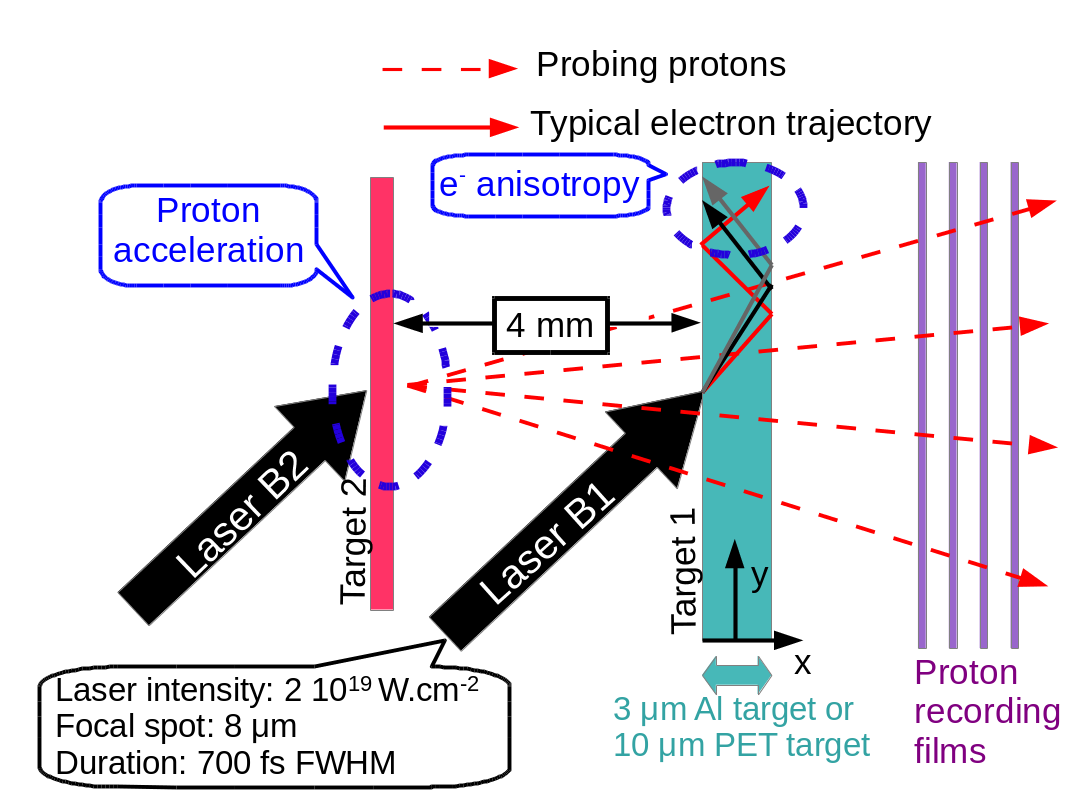
\includegraphics[scale=0.25]{sketch.png}\\
\end{tabular}}
\caption{\label{fig:xp} \textbf{Sketch of the experimental configuration and physical picture}. Target 1 is in red, target 2 in green.}
\end{figure}
The experimental and numerical data gathered so far seem to suggest that magnetic filaments only form relatively near the laser axis (over a few tens of microns), where the fast electron density, and therefore the overall plasma anisotropy, are initially at their highest. Furthermore, in contrast with simulation results \cite{POP_Heron_2015, POP_Yang_2016}, there has been as yet no observation of the simultaneous development of the collisionless and resistive variants of the instability in, respectively, the surface and inner regions of dense targets. 
Here we present measurements and simulations demonstrating: (i) filamentary magnetic-field generation by fast electrons over spatial (hundreds of microns) and temporal (tens of ps) scales much larger than previously thought possible; (ii) the simultaneous development of the collisionless and resistive types of filamentation in different areas of the target, allowing us to untangle the conditions for their occurrence.

Our measurements make use of the proton radiography technique (see Fig.~\ref{fig:xp} and Methods), by means of two high-temporal-contrast, short-pulse laser beams, B1 and B2. More details on the setup can be found in Ref.~\cite{RSI_Albertazzi_2015}.
B2 irradiates target 2 (a $3\,\rm \mu m$ thick Al or a $10\,\rm \mu m$ thick PET foil) at an angle of $31^\circ$ to the target normal (in the horizontal plane), while B1 generates the probing protons from target 1. Depending on target 2's material (Al being a conductor, PET being an insulator), two types of electromagnetic field patterns are observed to arise, which kinetic simulations indicate are induced by collisionless and resistive current filamentation instabilities. These are triggered as the fast electrons, respectively, recirculate in the low-density plasma expanding into the vacuum and drift away from the laser spot into the cold, solid-density target bulk. As will be detailed in Figs.~\ref{fig:pic} and \ref{fig:kxy}, such instabilities generate electromagnetic structures consistent with the experimental observations in the Al and PET foils in terms of field strength ($\sim 10\,\rm T$), wavelength ($\sim 100\,\rm \mu m$), as well as spatiotemporal evolution (instability triggered a few $100\,\rm \mu m$ away from the focal spot, $\sim 1\,\rm ps$ after the main laser drive).
%
\begin{figure*}[tbh!]
\begin{tabular}{cc}
%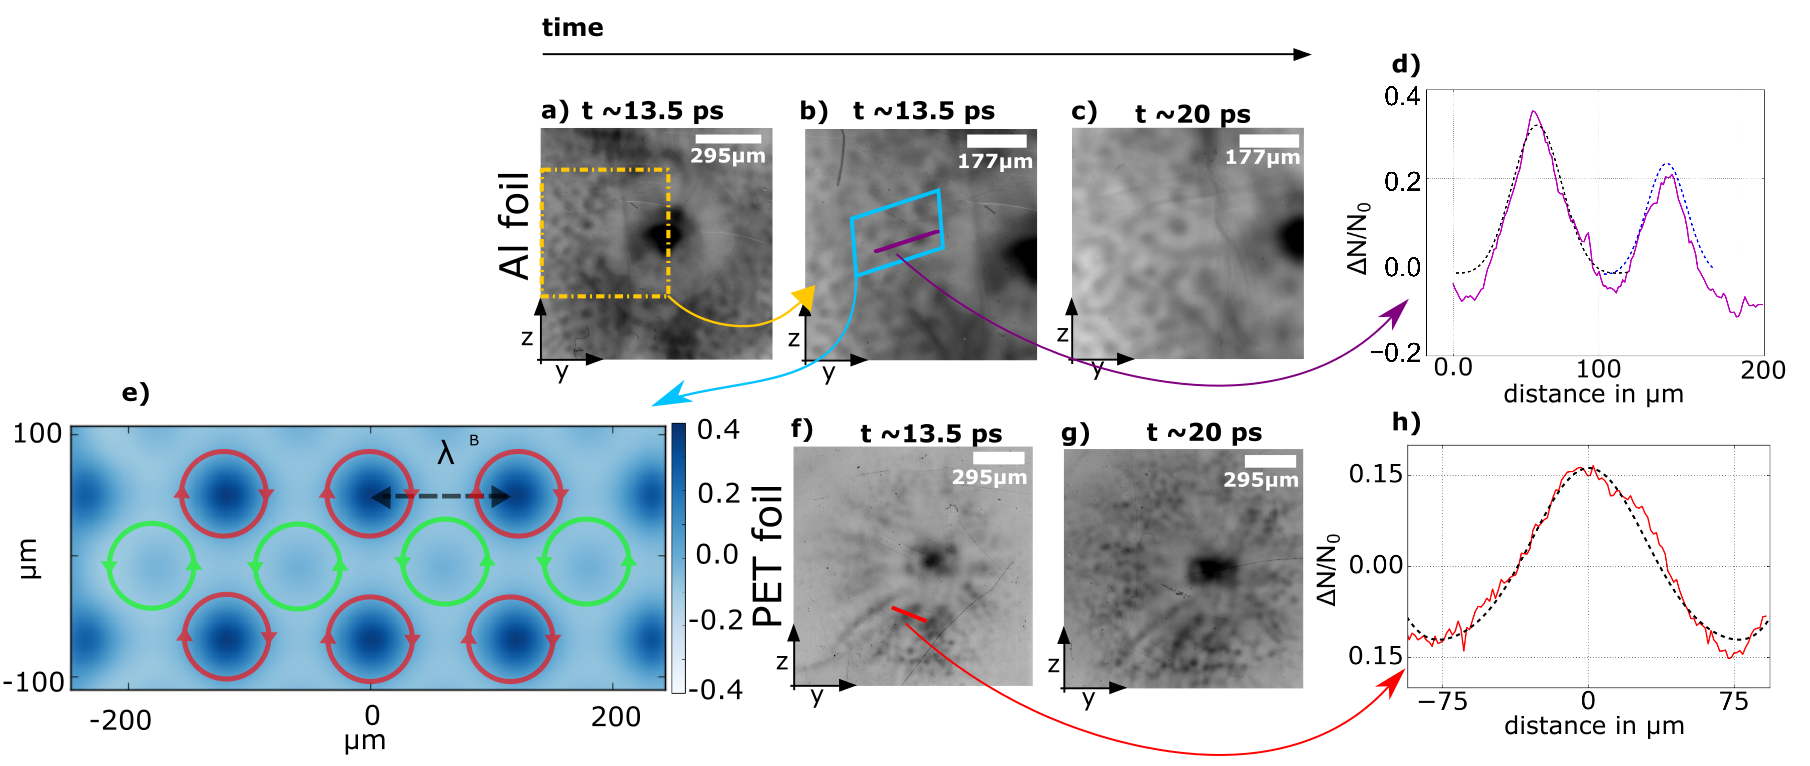
\includegraphics[scale = 0.6]{panel_v6.png}
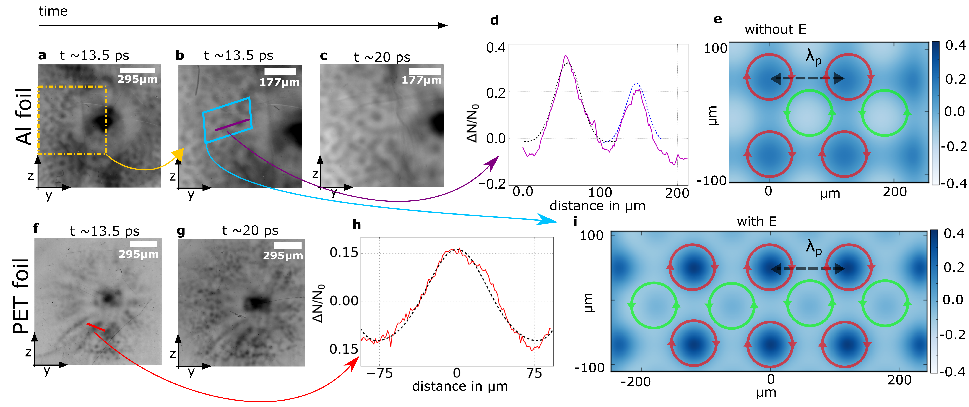
\includegraphics[width=0.99\textwidth]{panel_v7_woE2.png}
\end{tabular}
 \caption{
\textbf{Proton radiographs evidencing two types of filamentation instabilities driven by laser-generated hot electrons in metallic and dielectric targets}
%Experimental proton radiographs evidencing two types of filamentation instabilities driven by hot electrons generated in solid foils, and resulting electric and magnetic field patterns, depending on the initial electrical resistivity of the target. 
\textbf{a-c}, Radiographs at various times, obtained with an Al foil as target 2. $t=0$ refers to the time at which laser B2 irradiates target 2. Darker and lighter areas correspond to increased and depleted proton dose, respectively \cite{RSI_Albertazzi_2015}. 
\textbf{b-c}, Closeups of the off-center region delimited by the yellow dashed square in a. Small-scale modulations are observed to develop after $\sim 1\,\rm ps$.
%The small-scale modulations extending over the whole field of view are observed to develop after $\sim 1\,\rm ps$.
\textbf{d}, Normalized proton dose profile along the purple line in b (purple solid curve) and synthetic dose profiles (black and blue dotted curves) (see Methods).
\textbf{e}, Schematic pattern of the magnetic field lines (circular arrows) that could develop in the zone delimited by the blue box in b, overlaid on the resulting (simulated) proton dose modulation $\Delta N/N_0$ (pseudocolor map). Red and green loops indicate magnetic field lines of opposite polarity.
\textbf{f-g}, Proton radiographs obtained with a PET foil as target 2. On top of a small-scale dotted pattern akin to that seen in a-c, one observes radial streaks extending from the central laser spot. 
\textbf{h}, Normalized proton dose profile along the red line in f (red solid curve) and synthetic dose profile (black dotted line) (see Methods).
%All frames, for either the Al or PET foil, corresponding to different energies of the probing protons, and hence to different times-of-flight between target 1 and target 2 (as indicated above each frame), are taken from a single shot.
\textbf{i}, Same as e but considering the additional effect of the radial electric field induced in each pinched filament (see Methods and Supplementary Information).
All spatial scales refer to the target 2 plane.}
\label{fig:radio}
\end{figure*}

On the radiographs shown in Fig.~\ref{fig:radio}, the dark and white regions result from, respectively, accumulation and depletion of the probing protons through the quasistatic fields induced around target 2.
All frames associated with either the Al (Figs.~\ref{fig:radio}a-c) or PET (Figs.~\ref{fig:radio}f-g) foil, corresponding to different energies of the probing protons, and hence to different times-of-flight between target 1 and target 2 (as indicated above each frame), are taken from a single shot.
The irradiated region can be located by the large black area encircled by a white ring of $\sim 300\,\rm \mu m$ radius, delineating the large-scale $B$-field created by the Biermann battery on the surfaces of target 2 (see Ref.~\cite{RSI_Albertazzi_2015} and references therein). Remarkably, the radiographs also evidence a small-scale spotted pattern, developing from $\sim 400\,\rm\mu m$ to $\gtrsim 700\,\rm \mu m$ away from the focal spot, with a typical wavelength  $\lambda_p \simeq 100\,\rm \mu m$ (see lineout in Fig.~\ref{fig:radio}d). These structures, absent without B2 irradiating target 2 (the protons then exhibit a homogeneous dose, see Fig.~2i of Ref.~\cite{RSI_Albertazzi_2015}), are observed within the first ps following the laser peak (see first frame of Fig.~2a of Ref.~\cite{RSI_Albertazzi_2015}). Moreover, they are mainly located at the left-hand side of the irradiated region, \emph{i.e.}, in a domain towards which the hot electrons are expected to be preferentially flowing. Figure~\ref{fig:radio}e displays an idealized pattern of (azimuthal) magnetic and (radial) electric fields (see Methods), yielding a synthetic radiograph (pseudocolor map) qualitatively matching the experimental data. Note that the magnetic structures inferred in Ref.~\cite{PRL_Gode_2017} from modulations in the accelerated proton beam are consistent with what is observed in our radiographs, but with a much smaller wavelength and larger amplitude (due to their proximity to the laser spot).

The radiographs of the PET targets reveal a dotted pattern qualitatively similar to that seen in Al. Yet they also feature larger-scale radial dark streaks, which suggests that another mechanism for electromagnetic field generation, absent or weakly operative in Al, is here diagnosed on the line of sight of the probing protons.

\begin{figure*}[tbh!]
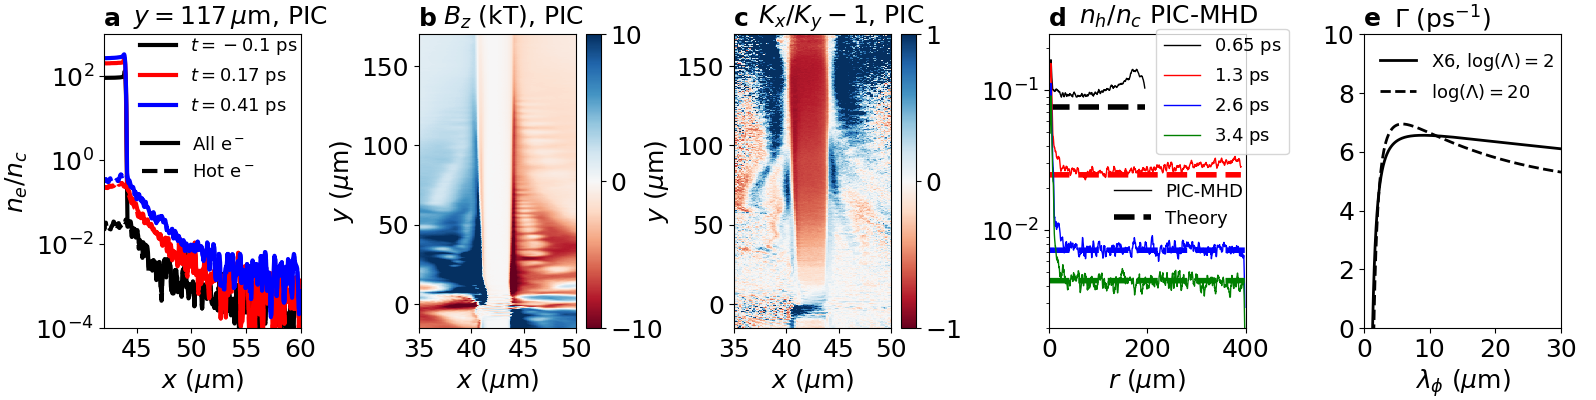
\includegraphics[scale=0.42]{Figure_3_new2.png}
\caption{
\textbf{\textcolor{red}{Kinetic numerical} simulations demonstrating the occurrence of plasma conditions favorable for the growth of the collisionless  and resistive current filamentation instabilities.}
\textbf{a}, \textbf{b}, \textbf{c}, Fully PIC 2D simulation of laser-plasma interaction in the $x-y$ plane (see Methods). 
\textbf{a}, Longitudinal lineouts at $y=117\,\rm \mu m$ of the total (solid lines) and hot ($E \ge 100\,\rm keV$, dashed lines) electron density (normalized to the critical density $n_c =1.1\times 10^{21}\,\rm cm^{-3}$) at different times, illustrating the hot-electron-driven plasma expansion along the target normal and away from the laser spot (located at $y=0$). \textcolor{blue}{In the expanding plasma ($x\gtrsim 44\,\rm \mu m$), the hot and total electron density profiles coincide.}
\textbf{b}, 2D map of the magnetostatic ($B_z$) field,  averaged over a laser cycle, at $t =0.41\,\rm ps$, showing \textcolor{red}{magnetic modulations} in the expanding plasma as the result of the collisionless Weibel instability.
\textbf{c}, Electron momentum-flux anisotropy, $K_x/K_y-1$, where $K_x$ (resp. $K_y$) is the local $x$ (resp. $y$) aligned momentum flux, averaged over electrons of energies $>100\,\rm eV$.
\textbf{d}, 2D PIC-MHD simulation of hot-electron transport in the $y-z$ plane (see Methods) with $T_{h0} = 1\,\rm MeV$, $T_{c0} = 50\,\rm eV$, $n_{h0} = 5 \times 10^{21}\,\rm cm^{-3}$, $R_0 = 32\,\rm \mu m$ and $\log \Lambda =2$. The simulated hot-electron density $n_h/n_c$ (solid lines), averaged poloidally around the \textcolor{red}{initial hot electron-filled area}, is plotted versus the radius $r=\sqrt{y^2+z^2}$ at different times, and compared with analytic estimates (dashed lines, see text).
\textbf{e}, Theoretical growth rate $\Gamma$ vs. poloidal wavelength $\lambda_\phi$ of the resistive current filamentation instability  (see Supplementary Information, Sec. III). Hot-electron parameters are extracted from PIC-MHD simulations run with $\log \Lambda = 2$, \emph{i.e.} modeling a conductor (solid line, multiplied by 6) and $\log \Lambda = 20$, \emph{i.e.} modeling an insulator (dashed line) at $t=0.5\,\rm ps$ [$n_h \simeq 2\times 10^{19}\,\rm cm^{-3}$, $T_x \simeq 300\,\rm keV$, $T_{ec} \simeq 500\,\rm eV$, $v_r=0$,  $T_\phi = 10\,\rm keV$ (resp. $13\,\rm keV$) for $\log \Lambda =2$ (resp. 20), see Methods].}
\label{fig:pic}
\end{figure*}

We will now show that the recirculation of the hot electrons across the dilute plasma expanding from the target surface triggers collisionless current filamentation, thus giving rise to electromagnetic structures such as those sketched in Fig.~\ref{fig:radio}e. In order to investigate the large-scale hot-electron dynamics in a self-consistent way, we have performed a 2D particle-in-cell (PIC) simulation using the code \textsc{calder} \cite{NF_Lefebvre_2003}. This simulation describes the laser-plasma interaction (and related collisional and ionization processes) in the $x-y$ plane shown in Fig.~\ref{fig:xp}, with half-reduced Al density to alleviate the computational effort (see Methods). Hereafter, the origin of time is placed when the pulse maximum reaches the target surface. We see in Fig.~\ref{fig:pic}a that, already at $t=0.41\, \rm ps$ (\emph{i.e.} $1.44\,\rm ps$ after injection of the laser pulse in the simulation), the rear target surface has moved a distance $>10\,\rm \mu m$, and that magnetic modulations have developed in the expanding plasmas from the two target sides (see Fig.~\ref{fig:pic}b and Supplementary Information, Figs.~S1 and S7). At the backside ($x>44\,\rm \mu m$), they extend up to $y \simeq 150\,\rm \mu m$ from the laser spot, with a typical wavelength $\lambda_p \simeq 6\,\rm \mu m$.

Electrons in the expanding plasma show a momentum-flux anisotropy $K_x/K_y - 1 \sim 1$ (where $K_x$ and $K_y$ are, respectively, the momentum fluxes along the $x$ and $y$ directions, see Figs.~\ref{fig:pic}c and S1f), suggesting that they are susceptible to the Weibel filamentation instability \cite{POP_Ren_2006, PRL_Gode_2017}. The growth rate and wavelength of the dominant mode can be estimated from the dispersion relation derived for an \emph{ad hoc} two-temperature relativistic distribution function
%\cite{POP_Yoon_2007a}
(see Supplementary Information, Sec.~II), the parameters of which are extracted from our fully PIC simulation. Moreover, the approximate magnetic-field wavelength and strength at saturation (see Supplemental information, Sec.~V.A) can be related to the hot-electron plasma frequency, $\omega_{ph}=\sqrt{n_h e^2/m_e \epsilon_0}$ and the electron thermal velocity $v_{hx}\sim 0.2c$ (see Fig.~S7c), through 
\begin{align}
  \lambda_p &\simeq \alpha_\lambda 2\pi c/\omega_{ph} \label{eq:lp}  \,,\\
  B_p &\simeq \alpha_\Gamma^2\alpha_\lambda m_e \omega_{ph}c/ ev_{hx} \label{eq:bp} \,, 
\end{align}
where $c$, $\epsilon_0$, $n_h$, $m_e$ and $e$ are the speed of light in vacuum, the vacuum permittivity, the hot electron density, the electron mass and charge, respectively. Also, $\alpha_\lambda $ and $\alpha_\Gamma $ are proportionality factors depending on the anisotropy and mean energy of the electron distribution; in our case, we have $\alpha_\lambda \sim 2$ and $\alpha_\Gamma\sim 0.1$ (see Supplementary Information, Sec. II, Fig.~S4).

\textcolor{red}{Far from the irradiated region, an electric field \mbox{$\mathbf{E_p} \simeq (\mathbf{J_h} \times \mathbf{B}-\nabla P_h)/(e n_h)$} should also build up ($\mathbf{J_h}$ and $P_h$ are, respectively, the hot-electron current density and pressure). A few picoseconds after the laser interaction, the pressure term, responsible from the Biermann battery effect, should be negligible, so that the electric field should originate from the pressure induced by the Weibel magnetic fluctuations, $\mathbf{E_p} \simeq - \nabla B_p^2/(2 \mu_0 e n_h)$. Physically, this field originates from charge separation in the Weibel filaments between the magnetically pinched electrons and the slowest-moving ions} \cite{POP_Dieckmann_2009, POP_Bret_Gremillet_2010}.
Its strength can be estimated using Eqs.~\eqref{eq:lp} and \eqref{eq:bp},
\begin{align} 
  E_p \simeq \alpha_\Gamma^4  \alpha_\lambda^2 m_ec^3\omega_{ph}/2ev_{hx}^2 \label{eq:ep} \, .
\end{align}
While the magnetic field around a filament tends to focus or defocus the probing protons depending on the filament's current sign, the accompanying electric field  is always focusing. The net effect on the proton deflection is determined by the modulation wavelength $\lambda_p$ (see Supplementary Information, Sec. V.B).

In order to demonstrate that the instability seen to grow in the simulated expanding plasma (Fig.~\ref{fig:pic}b) accounts for the dotted pattern evidenced by the radiographs (Fig.~\ref{fig:radio}), one needs to disentangle the impact of the reduced geometry of our simulation on the hot-electron dynamics. Indeed, unlike in Refs.~\cite{PRL_Gode_2017, NJP_Scott_2017}, field modulations here build up at least a picosecond after the laser irradiation, and hundreds of microns away from the focal spot, where multidimensional electron dilution effects should arise. Obviously, such effects are improperly treated in our fully PIC 2D simulation, which resolves only the $x-y$ plane. Yet they can be evaluated by estimating the temporal evolution of the hot-electron density, $n_h$, in a general system of spatial dimension $D+\delta$, where $D$ and $\delta$ denote the number of dimensions in the target plane and normally to it, respectively. Assuming a homogeneous spatial distribution, and taking into account both the transverse thermal spread of the hot electrons and the longitudinal plasma expansion, one obtains $n_h(t) \simeq \alpha_n n_{h0}/(1+ v_{hr} t /R_0)^D/(1+c_{sh} t/L)^\delta$ with $L$, $c_{sh}$, $n_{h0}$, $R_0$, $v_{hr}$, and $\alpha_n$ being the target thickness, sound speed, initial hot-electron density,  deposition radius, radial thermal velocity spread and proportion of spreading hot electrons, respectively. Our fully PIC simulation suggests that $R_0 \simeq 32\,\rm \mu m$, $n_{h0} \simeq 5\times 10^{21}\,\rm cm^{-3}$ (see Fig.~S3a).

To constrain the above values of $\alpha_n$ and $v_{hr}$, we have carried out a 2D PIC-MHD simulation resolving the hot-electron transport through the solid-density Al target in the transverse ($y-z$) plane. In this simulation, the laser-plasma interaction and longitudinal plasma expansion are not described, while the response of the thermal bulk electrons is modeled in the resistive MHD limit, which allows the hot electrons to be followed over larger spatiotemporal scales than in the fully PIC simulation (see Methods). At $t = 0$, the hot electrons are initialized as an isotropic Maxwellian population of temperature $T_{h0}=1\,\rm MeV$ and density $n_{h0}=5\times10^{21}\,\rm cm^{-3}$, contained in a circular region of radius $R_{0}=32\,\rm \mu m$. The initial Al plasma temperature is of $50\,\rm eV$, corresponding to a $5+$ ionization degree. Such input parameters are based on the fully PIC simulation data (see Supplementary Information, Sec. I).

The hot-electron density profiles extracted at various times from the PIC-MHD simulation (see Figs.~\ref{fig:pic}d and S7) support the above estimate for $n_h(t)$ (taking $D=2$ and $\delta=0$) with $\alpha_n \simeq 0.25$ and $v_{hr}\simeq 0.5c$ (see Supplementary Information, Sec.~IV.B). Also, taking $D=\delta=1$, our formula predicts $n_h \simeq 3.4 \times 10^{19}\,\rm cm^{-3}$ at $t=1.44\,\rm ps$, consistent with the fully PIC simulation (Fig.~\ref{fig:pic}a). Further, \textcolor{red}{Eqs.~\eqref{eq:lp} and \eqref{eq:bp} give $\lambda_p \simeq 11 \,\rm \mu m$ and $B_p \simeq 190\,\rm T$, close to the simulation data (see Fig.~\ref{fig:pic}b and Fig.~S1b). In this simulation, however, due to its reduced geometry and too short integration time, the magnetic field in the modulated region comprises comparable Weibel and Biermann-battery components, invalidating the electric field estimate Eq.~\eqref{eq:ep} (see Supplementary information Sec.~V.B).}

In the experimental geometry ($D=2$, $\delta=1$), keeping the above 2D values for $v_{hx}$, $\alpha_\lambda$ and $\alpha_\Gamma$, one obtains $n_h \simeq 2.7 \times 10^{17}\,\rm cm^{-3}$ and $\lambda_p \simeq 130\,\rm \mu m$ at $t=4\,\rm ps$, in fair agreement with the observed structures  (Figs.~\ref{fig:radio}a-c). A magnetic field strength $B_p \simeq 17\,\rm T$ is predicted, close to the experimentally inferred value of $\sim 10\,\rm T$ (see Methods). Moreover, the accompanying electric field is expected to be strong enough ($E_p \simeq 0.12 \,\rm GV.m^{-1}$) to affect the radiographs (see Fig.~\ref{fig:radio}i) by increasing (resp. fading) the contrast of the focusing (resp. defocusing) magnetic loops (see Supp. Info. Sec.~V). Since hot electron recirculation and target expansion occur on both sides of the target, the probing protons should form two overlaid, independent electromagnetic patterns on the detector (see Methods and supplementary information Sec. V.C). %Figures~\ref{fig:kxy}b,c display synthetic radiographs resulting from one scattering distributions (see Methods and discussion below). 

\begin{figure*}
\centerline{
\begin{tabular}{ccc}
\textbf{a} PIC-MHD magnetic field  &  \textbf{b} Synthetic radiograph   &  \textbf{c} Synthetic radiograph  \\
& without expanded plasma &   with expanded plasma \\
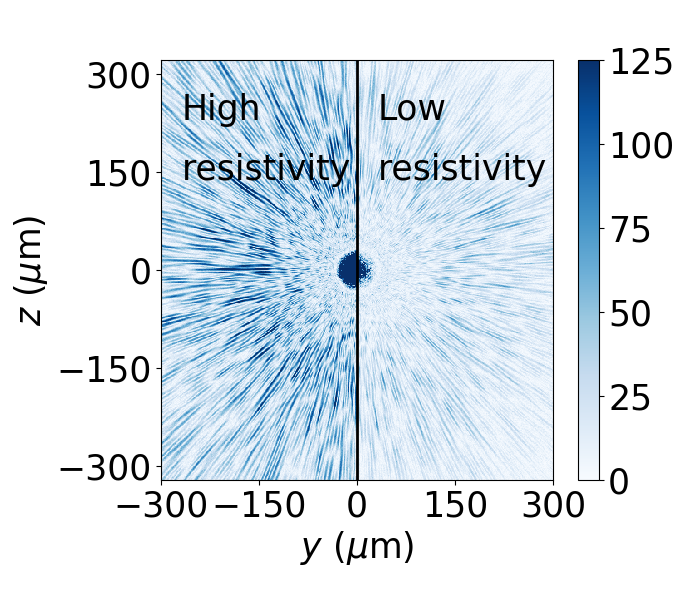
\includegraphics[scale=0.33]{B_Te0_05_ne300_nh5_Th1MeV_t10500_complog.png} &
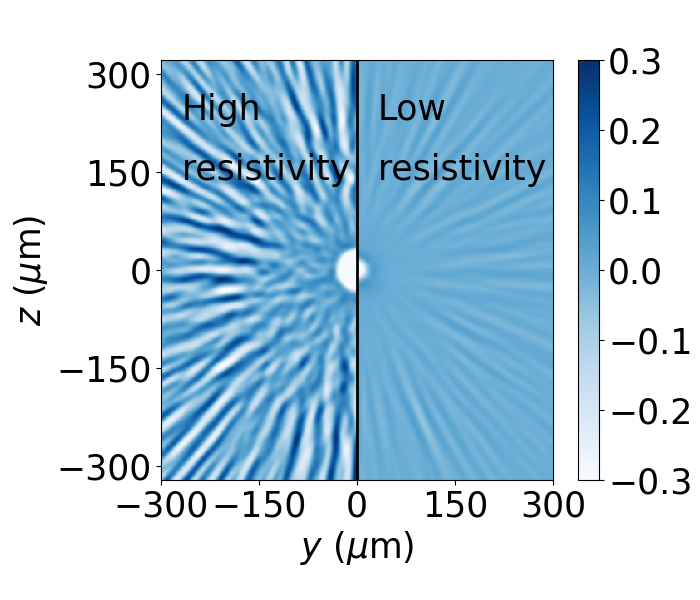
\includegraphics[width=0.33\textwidth]{DN_Te0_05_ne300_nh5_Th1MeV_t10500_complog_300mum.png} &
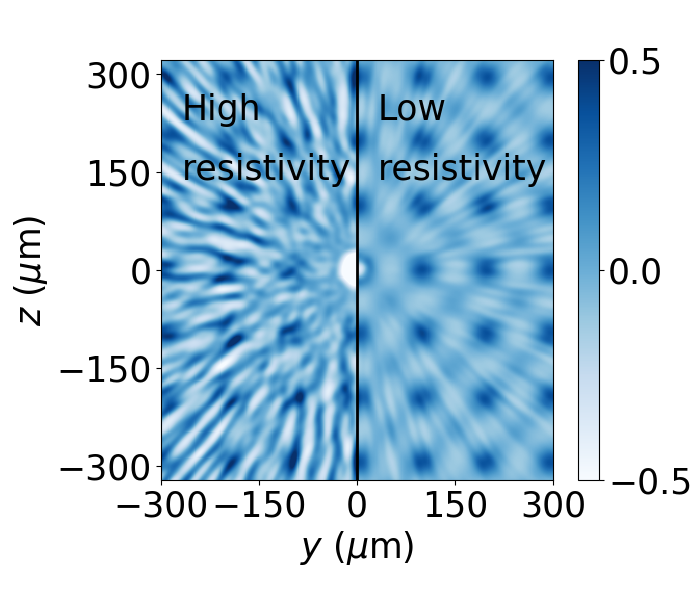
\includegraphics[width=0.33\textwidth]{DN3D_complog_R20_a60_l140.png}
\end{tabular}}
\caption{
\label{fig:kxy}
\textbf{2D PIC-MHD simulations evaluating the resistive filamentation growth in the solid foil plane for various initial electrical resistivities.}
\textbf{a}, Magnitude of $B_\perp=(B_x^2+B_y^2)^{1/2}$ (in Teslas) at time $t=3.28\,\rm ps$ for $\log \Lambda=20$ (\emph{i.e.} modeling an insulator, $y<0$) and $\log\Lambda=2$ (\emph{i.e.}, modeling a conductor, $y>0$).
\textbf{b}, Synthetic radiographs from $8\,\rm MeV$ probing protons in a 
$3\,\rm \mu m$ thick target with B-fields given by a (see Methods).
\textbf{c}, Synthetic radiographs with superimposed filaments extending in the $z$ direction over $L_p = 48\,\rm \mu m$ (see Methods).
Following Fig.~\ref{fig:radio}e, the magnetic field used for the reconstruction is taken to be poloidal around each filament center (of periodicity $\lambda_p = 140\,\rm \mu m$), and to obey the radial profile given by Eq.~\eqref{eq:bloop} with $B_0=10\,\rm T$ and $a = 60\,\rm \mu m$. One electromagnetic distribution has been placed on the expanding rear side of the $3\,\rm \mu m$ thick target (see Methods for details on their arrangement).}
\end{figure*}

The PIC-MHD simulations capture the lateral spreading dynamics of the hot electrons, and hence the resistive filamentation instability that can affect it. As the electrons move radially away from their generation region, their momentum distribution becomes ``cold'' in the poloidal ($\theta$) direction, while it stays ``hot'' along the other ($r,x$) directions (see Fig.~S6 in Supplementary Information Sec. IV.A). A large anisotropy in the hot electron pressure is therefore driven in $\sim 0.5\,\rm ps$, although its final level may be overestimated due to neglect of the longitudinal target expansion and of the associated electron-to-ion momentum-transfer (occurring after $\sim L/2c_{sh} \sim 0.5\,\rm ps$ \cite{PRE_Mora_2005}). Therefore, in the case of the conducting Al target (characterized by a Coulomb logarithm $\log \Lambda = 2$ \cite{POF_Lee_1984}), a non-propagating magnetic modulation builds up after a few $100\,\rm fs$ (see \mbox{Fig.~\ref{fig:kxy}a, right}), reaching a field strength $\langle B_\phi^2\rangle^{1/2}\simeq 34\,\rm T$ (averaged over the region $100 \ge r \ge 200\,\mu \rm m$) with a typical (poloidal) wavelength $\lambda_\phi \simeq 5-10\,\rm \mu m$. These results are compatible with the linear dispersion relation of the resistive filamentation instability, evaluated using parameters extracted from the PIC-MHD simulation at $t=0.5\,\rm ps$, and which predicts a fastest-growing wavelength $\lambda_\phi \simeq 5\,\mu \rm m$ (Fig.~\ref{fig:pic}e, see Supplemental Information Sec. III). The instability growth time, $\Gamma_\phi^{-1}\simeq 160\,\rm fs$ is also consistent with the experimental time of appearance of the proton dose modulations ($0-1\,\rm ps$ after laser irradiation).

We will now assess the influence of the target electrical resistivity on the observed radial structures. The hot-electron dynamics in the insulating PET target is expected to differ from that in the conducting Al target due to higher electrical resistivity at low temperatures \cite{PRL_Fuchs_2003, PRL_McKenna_2011}. Since our PIC-MHD framework ceases to be accurate outside the Spitzer collisional regime ($T\lesssim 50\,\rm eV$), we will restrict ourselves to a qualitative comparison by running the same simulation than in Al but with an artificially enhanced resistivity, \emph{i.e.}, using a Coulomb logarithm $\log \Lambda = 20$ instead of $\log \Lambda = 2$, so as to mimic the response of the PET bulk target electrons. Comparing the magnetic field maps displayed in the left and right-hand sides of Fig.~\ref{fig:kxy}a, one can see that about twice stronger field modulations ($\langle B_\phi^2 \rangle^{1/2} \simeq 70\,\rm T$ vs. $35\,\rm T$) build up at $\log \Lambda = 20$, while keeping approximately the same wavelength. This behavior is consistent with the dispersion relation of the resistive filamentation instability (see Methods and Supplemenatry Information). Indeed, from the simulation data in the region $50 \le r \le 100\,\rm \mu m$ (see Figs.~S6a-f), the maximum growth rate (dashed line in Fig.~\ref{fig:pic}e) is predicted to be $\sim 6$ times larger at $\log \Lambda = 20$ than at $\log \Lambda = 2$, with about the same wavelength. 

After saturation of the instability, the hot electrons' contribution to the magnetic structures progressively weaken due to dilution, so that the latter end up being sustained by the bulk thermal electrons only, thus being subject to magnetic diffusion over a timescale $\tau_d \simeq \mu_0 \sigma \lambda_\phi^2 \gtrsim 30\,\rm ps$ at temperatures $\gtrsim 50\,\rm eV$. Hence, we do not expect significant evolution of the fields inside the target over a $\sim \tau_d$ timescale following the final simulation time ($3.28\,\rm ps$).

Figures~\ref{fig:kxy}b,c display synthetic radiographs obtained from proton ray-tracing calculations through the field distributions extracted from the above simulations (see Methods). In Fig.~\ref{fig:kxy}b only the PIC-MHD fields are taken into account (for both $\log \Lambda =2$ and $\log \Lambda = 20$), while Fig.~\ref{fig:kxy}c further considers the effect of the electric and magnetic fluctuations that arise in the expanding plasma. In all cases, scattering of the probing protons off the target ions is also described (see Methods and Supplementary Information Sec. V), and is responsible for the smoothed rendering of Fig.~\ref{fig:kxy}b compared to Fig.~\ref{fig:kxy}a. In the low-resistivity (Al) target,  Figs.~\ref{fig:kxy}b,c show that the dotted field pattern induced in the expanding plasma mainly accounts for the observed proton modulations. In the high-resistivity (PET) target, by contrast, the field patterns generated both in the expanding plasma and the bulk target are found to contribute to the radiographs. The larger number of radial structures in the synthetic radiographs \textcolor{red}{(Figs.~\ref{fig:radio}f,g) is ascribed to the imperfect} modeling of the electrical resistivity of the target and to uncertainties in the initial hot electron parameters.

To conclude, we have shown, through proton radiography, that the energetic electrons generated by an intense short-pulse laser can induce quasistatic electromagnetic fluctuations of significant strength ($\sim 10\,\rm T$) at surprisingly large distances (a few hundreds of $\rm \mu m$) from the laser spot. Based on numerical kinetic simulations and theoretical estimates, our analysis reveals that two instability-based mechanisms for field generation can operate simultaneously, namely collisionless current filamentation in the expanding plasmas formed at the target surfaces, and resistive current filamentation in the bulk target. The former is found to prevail in conducting Al targets, while both yield comparable field strengths in high-resistivity PET targets. A full quantitative understanding of our experimental observations would require describing the multidimensional hot-electron kinetics in dense plasmas over tens of ps and hundreds of $\rm \mu m$ spatiotemporal scales. Not only out of reach of state-of-the-art kinetic simulation codes, this challenging problem also require progress in the theoretical modeling of the coupled-to-weakly-coupled plasma transition during laser irradiation.

\section*{Methods}
\subsection*{Experiments}
The experiment 
was performed at the Jupiter Laser Facility's \textsc{titan} laser at the Lawrence Livermore National Laboratory \cite{RSI_Albertazzi_2015}. Each laser beam B1 and B2 had an energy of $55\,\rm J$ ($\pm 10\%$), a pulse duration of $\sim 700\,\rm fs$ FWHM, and was focused with a $f/3$ parabola at $31^\circ$ incidence angle in the horizontal plane, resulting in an on-target intensity of $\sim 2\times 10^{19}$ W.cm$^{-2}$. The normalized laser field strength was $A_0 = eE/m_ec\omega_0 \simeq 4$, where $\omega_0$ is the laser frequency. Before focusing, B2 was reflected off a plasma mirror, with $70\,\%$ efficiency, in order to improve its temporal contrast \cite{PRE_Doumy_2004}. A high temporal contrast ensured steep density gradients at the target surface, which is critical for the formation and observation of the far-distant magnetic loop structures revealed here (\emph{e.g.}, compare with the results of Ref.~\cite{PRL_Sarri_2012} where no similar structures were observed, likely due to the generation of a large preplasma by the laser prepulse). 

The probing protons, generated through target normal sheath acceleration \cite{PRL_Fuchs_2003} by focusing B1 onto a $50\,\rm \mu m$-thick Au foil, had a useful energy range of $4.5\,\rm MeV$ to $9.5\,\rm MeV$. They probed the $B$-fields developing in target 2 in a ``face-on'' configuration \cite{RSI_Albertazzi_2015}, suited to measuring toroidal magnetic loops having their axis along the target normal, while minimizing the influence of the $E$-fields that develop along the target normal. As shown in Fig.~\ref{fig:xp}, the probing protons, after propagation through target 2, were collected by a stack of radiochromic films \cite[]{RSI_Chen_2016} in which they were stopped in distinct layers according to their incident energy. Time-of-flight differences between protons of various energies from their source up to target 2 allowed us to probe the central, large-scale, as well as the radially distant, smaller-scale, electromagnetic fields at successive times ($t=0$ corresponds to the time at which B2 strikes target 2). Target 2 was either a $3\,\rm \mu m$-thick Aluminum (Al) foil or a $10\,\rm \mu m$-thick Polyethylene terephthalate [PET, an insulator polymer with composition $(\mathrm{C}_{10}\mathrm{H}_8\mathrm{O}_4)_n$].
 
\subsection*{2D fully PIC simulation}

A large-scale PIC simulation (2D in space, 3D in momentum) of the irradiation of the Al foil by the laser beam B2 has been performed using the PIC code \textsc{calder} \cite{NF_Lefebvre_2003}. The laser beam has a Gaussian temporal profile of $690\,\rm fs$ FWHM, a Gaussian spatial profile of $8\,\rm \mu m$ FWHM and a $30^\circ$ incidence angle. Its maximum intensity is of $3.5 \times 10^{19}\,\rm W.cm^{-2}$, reached at $t=0\,\rm ps$ on the target surface. The simulation unfolds between $t = -1.03\,\rm ps$ and $t = 0.41\,\rm ps$. The target is composed of three layers: H$^+$ ($0.7\,\rm \mu m$), Al$^{3+}$ ($3.7\,\rm \mu m$) and neutral hydrogen ($6\,\rm nm$). Its density profile consists of a $3\,\rm \mu m$ long plateau preceded by a $1.4\,\rm \mu m$-long preplasma made of H$^+$ and Al$^{3+}$ ions. The maximum ion target density is taken to be half the solid density ($n_\mathrm{Al}=n_\mathrm{H}=90 n_c$) so as to reduce the computational load. All species are initialized with a temperature of $10\,\rm eV$.

The numerical box has dimensions $L_x \times L_y = 83.5 \times 389.9\,\rm \mu m^2$ with a spatial discretization $\Delta x = \Delta y = 5.6\,\rm nm$ and a time step $\Delta t = 1.48\times 10^{-2}\,\rm fs$. An alternating-order interpolation scheme \cite{CPC_Sokolov_2013} is employed with a 4th-order weight factor. Each cell initially contains 50 macro-particles per species in the Al layer and 500 macro-particles per species in the thin H layers. The Maxwell solver proposed in Ref.~\cite{PRSTAB_Lehe_2013} is used along with a combination of spatial \cite{JCP_Vay_2011} and temporal \cite{JCP_Friedman_1990} filtering. Elastic Coulomb collisions, electron impact ionization and field ionization are modeled following Refs.~\cite{POP_Perez_2012}.

\subsection*{2D PIC-MHD simulations}

In order to access spatiotemporal scales of experimental relevance in a 2D geometry, we have employed the resistive magnetohydrodynamic PIC model proposed in Ref.~\cite{JCP_Cohen_2010}. This numerical scheme, implemented into the code \textsc{calder} \cite{NF_Lefebvre_2003}, consists in replacing the Maxwell-Amp\`ere equation by the generalized Ohm's law
\begin{equation} \label{eq:PICMHD}
  \mathbf{E}=\eta \left(\nabla \times \mathbf{B}-\mathbf{J}_h-\frac{\partial \mathbf{E}}{\partial t}\right)+\frac{\mathbf{J}_c\times \mathbf{B}}{en_c}
  -\frac{\nabla P_c}{en_c} \,,
\end{equation}
where $\eta$ is the electrical resistivity, $n_c$, $P_c$ and $\mathbf{J}_c$ are the density, pressure and current density of the thermal (`cold') electrons and $\mathbf{J}_h$ is the current density of the hot electrons. Since this scheme only accounts for the generation of non-radiative fields, it allows one to use mesh sizes (resp. time steps) much larger than the plasma skin depth (resp. plasma period), thus greatly alleviating the computational load. In a given cell, electrons are considered `cold' if their velocity fulfills $v<5\sqrt{T_c/m_e}$, where $T_c$ is the local temperature of the cold electron population at the previous time step; the remaining electrons are considered `hot'.

Our PIC-MHD simulation (2D in space and 3D in momentum) self-consistently describes the evolution of an initially confined source of hot electrons through a dense Al plasma in the $y-z$ plane parallel to the target surface (assuming invariance along the $z$ axis). Initially, the hot electrons uniformly fill a cylinder of radius $R_{0}$=$32\,\rm \mu m$  with a density $n_{h0}=5\times 10^{21}\,\rm cm^{-3}$, centered around $(y,z)=(0,0)$. 
The start time of the simulation is assumed to correspond approximately to the time of the laser pulse although the time-dependent hot-electron generation is not described.
The choice of an initial hot-electron source wider than the $\sim 8\,\rm \mu m$ laser spot partly accounts for the radial expansion of the hot electrons during the laser pulse \cite{PRE_Stephens_2004} (thus ensuring a relatively moderate $n_{h0}$, as is expected). Their momenta are distributed according to an isotropic Maxwell-J\"uttner distribution of temperature $T_{h0}=1\,\rm MeV$. Simulations performed with different initial temperatures (from $200$ to $500\,\rm keV$) or anisotropic distributions (with $T_x>T_{y,z}$) yield qualitatively similar results. The total kinetic energy carried by the hot electrons is $\sim 25\,\rm J$, which amounts to $\sim 50\%$ of the B2 laser energy \cite{PRL_Ping_2008}. The hot-electron spot is immersed inside a solid-density Al$^{5+}$ plasma of \mbox{50-eV} temperature. The bulk (`cold') electron density is $n_{c0}=300n_c$ everywhere, except within the hot spot, where it reduces to $n_{c0}=295n_c$ to ensure charge neutrality. Coulomb binary collisions between all the charged particle species and impact ionization of the Al ions are described using the framework of Ref.~\cite{POP_Perez_2012}. The electrical resistivity involved in Ohm's law is calculated in the Spitzer regime with the numerical fits given in Ref.~\cite{Decoster_1998}. 

The computational domain has dimensions
$L_x\times L_y=800 \times 800\,\rm \mu m^2$ and is discretized with mesh sizes $\Delta x=\Delta y =0.16\,\rm \mu m$. The time step is $\Delta t=0.34\,\rm fs$. The boundary conditions are taken to be absorbing for the particles and reflective for the fields. The ion and cold electron populations are initially modeled by 100 macroparticles per cell, while the hot electrons are modeled by 1000 macroparticles per cell. 

%Since, in our study, the PIC-MHD scheme aims at modeling the streaming of the fast electrons and not the laser energy deposition dynamics, the simulation starting time lies around $t = 0$ (\emph{i.e.} the moment the maximum laser intensity reaches the target surface). As our numerical results extend over $3.28$ ps, the temporal domain covered by our simulation is $0 < t < 3.28\, \rm ps$, although a vagueness formally remains over the initial date due to the finite duration of the laser pulse. 

\subsection*{Theory of the resistive filamentation instability}

The dispersion relation of the filamentation instability driven by hot electrons streaming through a dense resistive plasma has been derived within a kinetic-fluid framework, similarly to Ref.~\cite{POP_Gremillet_2002}. The hot electrons are taken to obey a two-temperature Maxwellian distribution (neglecting relativistic effects for simplicity), and their perturbed current density is obtained from the linearized Vlasov equation. The cold bulk electron current is given by the simple Ohm's law $\mathbf{J}_c=\sigma \mathbf{E}$.
After some algebra and a third-order Taylor expansion of the linear dispersion relation, one can estimate the growth rate as a function of the fluctuation wavenumber (see Supplementary Information). The input electron parameters have been extracted from the PIC-MHD simulations. For $\log \Lambda=2$ and at $t=0.5\,\rm ps$ (Fig.~\ref{fig:kxy}a, right), the hot-electron density ($n_h$) and poloidal/longitudinal temperatures ($T_{\theta/x}$) are measured to be $n_h\simeq 0.02 \times 10^{21}\,\rm cm^{-3}$, $T_\theta \simeq 10\,\rm keV$ and $T_x= 300\,\rm keV $ (see dashed black lines in Figs.~S5a-e). For $\log \Lambda =20$, (Fig.~\ref{fig:kxy}a, left), one has $n_h \simeq 0.02 \times 10^{21}\,\rm cm^{-3}$,  $T_\theta \simeq 13\,\rm keV$ and $T_x \simeq 300\,\rm keV$. The cold-electron radial drift velocity ($v_r$) and temperature ($T_c$) are found to vary in the ranges $0\lesssim \vert v_r \vert \lesssim 2\times 10^8 \,\rm m.s^{-1}$ (see Fig.~S5c) and $150 \lesssim T_c \lesssim 600\,\rm keV$ (see Fig.~S6b). The curves plotted in Fig.~\ref{fig:pic}e correspond to $v_r = 0$ and $T_c=500\,\rm eV$.
Increasing $v_r$ up to $2\times 10^8 \,\rm m.s^{-1}$ or decreasing $T_c$ to $150\,\rm eV$ enhances the maximum growth rate, yet does not change the qualitative ordering of the low- and high-resistivity curves (plain and dashed lines in Fig.~\ref{fig:pic}e).

\subsection*{Synthetic radiographs}
The synthetic proton radiographs displayed in Fig.~\ref{fig:kxy} have been generated using the \textsc{ilz} program developed at LULI. This numerical tool allows us to confront the kinetic simulation results with the experimental data (Fig.~\ref{fig:radio}), and hence to infer the topology of the proton-probed magnetic fields.

\textsc{ilz} computes numerically the proton trajectories in a given stationary electromagnetic distribution, neglecting collective effects. 
%Each trajectory is computed independently so that collective effects are neglected. This assumption is based on the very high laminarity of the laser-accelerated protons \cite{PRL_Cowan_2004, PRL_Fuchs_2003} when using, like here, a high-Z (Au) foil as the proton source, meaning that the proton source size is very small ($\mu$m-scale) and that there is no proton trajectory crossing. (collective effects $\ne$ trajectory crossings!)
%The electromagnetic  fields  initialized by the user, are interpolated at the 0th up to the 2nd order and assumed static, which is reasonable regarding the short time-scale of the proton crossing time through the plasma ($0.15\,\rm ps$, since the protons are of several MeV energy for the proton radiography presented in this paper) with respect to the typical magnetic field time-scale ($\sim 0.5\,\rm ns$, as given by the Alfv\'en velocity). The charged particle motion through the electromagnetic  field structure is resolved with the Boris “leap frog” algorithm, which conserves the energy. \textcolor{red} Ces details me semblent superflus. De plus, on se contredit quelque peu en attribuant ici la dynamique des champs a la vitesse d'Alfven alors que precedemment on invoque la diffusion magnetique.}
The input proton flux is taken to be monoenergetic with a uniform angular distribution within an emission lobe \textcolor{red}{broad enough  ($>8^\circ$)} to probe the whole PIC-MHD simulation plane. The dose variation onto the detector plane is evaluated as $\Delta N/N_0= (N-N_0)/N_0$, where $N_0$ and $N$ are the locally measured fluxes (in a given solid angle) before and after crossing the electromagnetic distribution. Owing to the small areal density of the target, the collisional energy loss of the protons can be neglected. Their collisional angular scattering is simply modeled by convolving the dose variation with a Gaussian of rms width corresponding to the angular spread \cite{NIM_Highland_1975}:
\begin{equation}
\theta_{1/e}  = \frac{E_s}{p\beta c} \sqrt{\frac{L}{L_R}} \epsilon \,,
\end{equation}
where $L$ is the target thickness, $L_R$ is the radiation length of the material, $p$ is the incident proton momentum, $\epsilon  = 1 + 0.038 \log\left(L/L_R\right)$ is a correction term \cite{EPJ_Groom_2000}, and $E_s=13.6\,\rm MeV$ is a constant.

We have considered a magnetic field distribution composed of a periodic array of magnetic loops of interspacing $\lambda_p$. Each loop obeys the following radial profile,
\begin{equation}\label{eq:bloop}
B_\theta(r)  = \pm \frac{B_0 r}{a} \frac{ e^{-r^2/a^2} }{\mathrm{max}_x(xe^{-x^2})} \,,
\end{equation} %Note : \mathrm{max}_x(xe^{-x^2}) = 0.42888
with $a$ being the radial size of the structure and $B_0$ its maximum field strength. The magnetic field distribution is assumed to comprise magnetic loops of opposite polarity, as drawn in Fig.~\ref{fig:radio}e (the colormap depicts the \textsc{ilz}-computed proton dose variation). 

The electric field associated with each magnetic loop has been estimated by balancing its resulting force on the plasma electrons and the magnetic pressure force, giving $E_r = -\nabla B^2 /(2\mu_0e n_e)$ \cite{POP_Dieckmann_2009, POP_Bret_Gremillet_2010}. Using Eq.~\eqref{eq:bloop} leads to the expression
\begin{equation}\label{eq:eloop}
E_r(r) = -\frac{  eB_0^2\lambda_p^2   e^{-2r^2/a^2}}{4\pi^2 m_e [\mathrm{max}_x(xe^{-x^2})]^2} \left[ \frac{r}{a^2}\left( 1-\frac{2r^2}{a^2}\right)  \right]  \,.
\end{equation} 

The modulations of the proton dose deposited in the RCF have been evaluated from the calibration performed in Ref.~\cite{RSI_Chen_2016}. The reference dose (from the non-deflected protons) has been measured outside of the modulated area. We have inferred the field parameters $a$ and $B_0$ from fitting the synthetic dose modulations to the data. Figure~\ref{fig:radio}d illustrates this procedure in the Al case: the two locally best-matching synthetic dose profiles, corresponding to $a=60\,\rm \mu$m and $B_0=10\,\rm T$ (black dotted line) and $a=34\,\rm \mu$m and $B_0=7\,\rm T$ (blue dotted line), are overlaid on the experimental profile (purple solid line). Figure~\ref{fig:radio}h exemplifies the PET case: here the experimental curve (red solid line) is well reproduced modeling the $B$-field locally as Gaussian, $B(r) = B_0 e^{-r^2/a^2}$, taking $a=40\, \rm \mu m$ and $B_0 = 40\,\rm T$ (black dotted line).

The electromagnetic field distribution underpinning the synthetic proton images shown in Fig.~\ref{fig:kxy}c consists in the juxtaposition of the electromagnetic loops detailed just above (placed at the rear side of the target) and the electromagnetic field map extracted from the PIC-MHD simulation. In other terms, in the \textsc{ilz} simulation, the protons first probe the fields predicted by the PIC-MHD simulation, and then the electromagnetic loops formed in the expanding plasma at the target backside.
The thickness of the expanding plasma has been taken equal to $c_s t \simeq 48\,\rm \mu m$,where $t\simeq 4\, \rm ps$ is the probing time. For completeness, the synthetic radiographs obtained by placing electromagnetic loops on both target sides are illustrated and examined in Fig. S10 of the Supplementary Information. 
%}

\begin{acknowledgments}
The authors gratefully acknowledge F.~Amiranoff, F.~Fiuza, E.~d'Humi\`eres, V.~Gubchenko, and V.T.~Tikhonchuk for insightful discussions.
We acknowledge the support of the JLF-Titan technical teams.
The simulations were performed using HPC resources at TGCC/CCRT. We acknowledge PRACE for awarding us access to TGCC/Curie (Grant No. 2014112576).
This project has received funding from the European Union’s Horizon 2020 research and innovation program under grant agreement no 654148 Laserlab-Europe and from the European Research Council (ERC) under the European Union’s Horizon 2020 research and innovation programme (grant agreement No 787539).
The research leading to these results is supported by Extreme Light Infrastructure Nuclear Physics (ELI-NP) Phase I, a project co- financed by the Romanian Government and European Union through the European Regional Development Fund. This work was partly done within the LABEX Plas@Par project. It was supported by Grants No. 11-IDEX-0004-02 and ANR-17-CE30-0026-Pinnacle from Agence Nationale de la Recherche. This work was also partly supported by the DFG GRK 1203 and SFB/TR18 programs and by EPSRC grants EP/K022415/1 \& EP/J002550/1. M.B. acknowledges co-financing by the European Social Fund and the state budget of the Czech Republic (project numbers CZ.1.05/1.1.00/483/02.0061 \& CZ.1.07/2.3.00/20.0279). 
This work was supported in part by the Ministry of Education and Science of the Russian Federation under Contract No.14.Z50.31.0007.
The use of the Jupiter Laser Facility  was supported by the U.S. Department of Energy, Lawrence Livermore  National Laboratory, under Contract No. DE-AC52-07NA27344.
\end{acknowledgments}

\section*{Author contributions}
JF conceived the project. BA, SNC, PA, JB, VD, LL, MN, LR, MSw, MB, HP and JF performed the experiment, with support from RS, OW and MSt.  BA, SB and JF analyzed the data. CRu and LG developed the theoretical framework and performed the simulations, with discussions with MG and CRi. SB computed the synthetic proton radiographs. JF, CRu and LG wrote the paper. All authors commented on the paper at its various stages.

%\textcolor{red}{
%Open questions, todo list:
%\begin{itemize}
%\item \textcolor{blue}{ Influence of electric field on the measurements $\rightarrow ok $ }
%\item \textcolor{blue}{ Demonstrate/justify the $B$-field topology in the expanding plasma $\rightarrow ok $ }
%\item \textcolor{blue}{Justify the neglect of the plasma expansion in the hot electron dilution modeling $\rightarrow ok $ }
%\item  \textcolor{blue}{ Temporal evolution of the B field in the expanded plasma: early time preferential location in accordance with the laser orientation $\rightarrow$ in Supplementary Information and the response to the referee}
%\item  \textcolor{blue}{ What is happening/ expected at late times ? $\rightarrow $done at the end }
%\item  \textcolor{blue}{ Smoothing effect in simulated radiographs $\rightarrow ok $}
%\item Relativistic effects in the hot electron dynamics
%\item Streaming vs. pressure anisotropy
%\end{itemize}
%}

%\textcolor{red}{
%Referee requirements, cf Answer to the referee
%\begin{itemize}
%\item Name of the instability Weibel vs. fiamentation
%\item field nature, electric field ?
%\item No occurance of "thermalization"
%\item Inclination of the laser
%\item correct former Ref 19
%\item Add ref to Schoeffler PRL and new PRE 2018
%\end{itemize}
%}

\bibliographystyle{naturemag}
%\bibliography{biblio}
\begin{thebibliography}{10}
\expandafter\ifx\csname url\endcsname\relax
  \def\url#1{\texttt{#1}}\fi
\expandafter\ifx\csname urlprefix\endcsname\relax\def\urlprefix{URL }\fi
\providecommand{\bibinfo}[2]{#2}
\providecommand{\eprint}[2][]{\url{#2}}

\bibitem{Shkarofsky_1966}
\bibinfo{author}{Shkarofsky, I.}, \bibinfo{author}{Johnston, T.} \&
  \bibinfo{author}{Bachynski, M.}
\newblock \emph{\bibinfo{title}{The Particle Kinetics of Plasmas}}
  (\bibinfo{publisher}{Addison-Wesley Pub. Co.}, \bibinfo{year}{1966}).

\bibitem{Belmont_2013}
\bibinfo{author}{{Belmont}, G.}, \bibinfo{author}{Roland, G.},
  \bibinfo{author}{Mottez, F.}, \bibinfo{author}{Pantellini, F.} \&
  \bibinfo{author}{Pelletier, G.}
\newblock \emph{\bibinfo{title}{{Collisionsless plasmas in astrophysics}}}
  (\bibinfo{publisher}{Wiley}, \bibinfo{year}{2013}).

\bibitem{Davidson_1983}
\bibinfo{author}{Davidson, R.~C.}
\newblock \bibinfo{title}{Kinetic waves and instabilities in uniform plasmas}.
\newblock In \bibinfo{editor}{Rosenbluth, M.~N.} \& \bibinfo{editor}{Galeev,
  R.~Z.} (eds.) \emph{\bibinfo{booktitle}{{Handbook of Plasma Physics}}},
  vol.~\bibinfo{volume}{1} (\bibinfo{publisher}{North-Holland},
  \bibinfo{address}{Amsterdam}, \bibinfo{year}{1983}).

\bibitem{PRL_Weibel_1959}
\bibinfo{author}{Weibel, E.~S.}
\newblock \bibinfo{title}{Spontaneous growing transverse waves in a plasma due
  to an anisotropic velocity distribution}.
\newblock \emph{\bibinfo{journal}{Phys. Rev. Lett.}}
  \textbf{\bibinfo{volume}{2}}, \bibinfo{pages}{83--84} (\bibinfo{year}{1959}).

\bibitem{POF_Fried_1959}
\bibinfo{author}{Fried, B.~D.}
\newblock \bibinfo{title}{Mechanism for instability of transverse plasma
  waves}.
\newblock \emph{\bibinfo{journal}{Phys. Fluids}} \textbf{\bibinfo{volume}{2}},
  \bibinfo{pages}{337--337} (\bibinfo{year}{1959}).

\bibitem{POF_Davidson_1972}
\bibinfo{author}{Davidson, R.~C.}, \bibinfo{author}{Hammer, D.~A.},
  \bibinfo{author}{Haber, I.} \& \bibinfo{author}{Wagner, C.~E.}
\newblock \bibinfo{title}{Nonlinear development of electromagnetic
  instabilities in anisotropic plasmas}.
\newblock \emph{\bibinfo{journal}{Phys. Fluids}} \textbf{\bibinfo{volume}{15}},
  \bibinfo{pages}{317} (\bibinfo{year}{1972}).

\bibitem{PRL_Lee_1973}
\bibinfo{author}{{Lee}, R.} \& \bibinfo{author}{{Lampe}, M.}
\newblock \bibinfo{title}{{Electromagnetic Instabilities, Filamentation, and
  Focusing of Relativistic Electron Beams}}.
\newblock \emph{\bibinfo{journal}{Phys. Rev. Lett.}}
  \textbf{\bibinfo{volume}{31}}, \bibinfo{pages}{1390--1393}
  (\bibinfo{year}{1973}).

\bibitem{PRL_Adam_2006}
\bibinfo{author}{Adam, J.~C.}, \bibinfo{author}{H\'{e}ron, A.} \&
  \bibinfo{author}{Laval, G.}
\newblock \bibinfo{title}{Dispersion and transport of energetic particles due
  to the interaction of intense laser pulses with overdense plasmas}.
\newblock \emph{\bibinfo{journal}{Phys. Rev. Lett.}}
  \textbf{\bibinfo{volume}{97}}, \bibinfo{pages}{205006}
  (\bibinfo{year}{2006}).

\bibitem{RPP_Marcowith_2016}
\bibinfo{author}{{Marcowith}, A.} \emph{et~al.}
\newblock \bibinfo{title}{{The microphysics of collisionless shock waves}}.
\newblock \emph{\bibinfo{journal}{Rept. Prog. Phys.}}
  \textbf{\bibinfo{volume}{79}}, \bibinfo{pages}{046901}
  (\bibinfo{year}{2016}).

\bibitem{APJ_Schlickeiser_2003}
\bibinfo{author}{{Schlickeiser}, R.} \& \bibinfo{author}{{Shukla}, P.~K.}
\newblock \bibinfo{title}{{Cosmological Magnetic Field Generation by the Weibel
  Instability}}.
\newblock \emph{\bibinfo{journal}{Astrophys. J. Lett.}}
  \textbf{\bibinfo{volume}{599}}, \bibinfo{pages}{L57--L60}
  (\bibinfo{year}{2003}).

\bibitem{PRL_Allen_2012}
\bibinfo{author}{Allen, B.} \emph{et~al.}
\newblock \bibinfo{title}{Experimental study of current filamentation
  instability}.
\newblock \emph{\bibinfo{journal}{Phys. Rev. Lett.}}
  \textbf{\bibinfo{volume}{109}}, \bibinfo{pages}{185007}
  (\bibinfo{year}{2012}).

\bibitem{PRL_Fox_2013}
\bibinfo{author}{Fox, W.} \emph{et~al.}
\newblock \bibinfo{title}{Filamentation instability of counter-streaming
  laser-driven plasmas}.
\newblock \emph{\bibinfo{journal}{Phys. Rev. Lett.}}
  \textbf{\bibinfo{volume}{111}}, \bibinfo{pages}{225002}
  (\bibinfo{year}{2013}).

\bibitem{NP_Huntington_2015}
\bibinfo{author}{Huntington, C.~M.} \emph{et~al.}
\newblock \bibinfo{title}{Observation of magnetic field generation via the
  {Weibel} instability in interpenetrating plasma flows}.
\newblock \emph{\bibinfo{journal}{Nat. Phys.}} \textbf{\bibinfo{volume}{11}},
  \bibinfo{pages}{173--176} (\bibinfo{year}{2015}).

\bibitem{PNAS_Mondal_2012}
\bibinfo{author}{Mondal, S.} \emph{et~al.}
\newblock \bibinfo{title}{Direct observation of turbulent magnetic fields in
  hot, dense laser produced plasmas}.
\newblock \emph{\bibinfo{journal}{Proceedings of the National Academy of
  Sciences}} \textbf{\bibinfo{volume}{109}}, \bibinfo{pages}{8011--8015}
  (\bibinfo{year}{2012}).

\bibitem{PRL_Romagnani_2019}
\bibinfo{author}{Romagnani, L.} \emph{et~al.}
\newblock \bibinfo{title}{Dynamics of the electromagnetic fields induced by
  fast electron propagation in near-solid-density media}.
\newblock \emph{\bibinfo{journal}{Phys. Rev. Lett.}}
  \textbf{\bibinfo{volume}{122}}, \bibinfo{pages}{025001}
  (\bibinfo{year}{2019}).

\bibitem{POP_Gremillet_2002}
\bibinfo{author}{Gremillet, L.}, \bibinfo{author}{Bonnaud, G.} \&
  \bibinfo{author}{Amiranoff, F.}
\newblock \bibinfo{title}{Filamented transport of laser-generated relativistic
  electrons penetrating a solid target}.
\newblock \emph{\bibinfo{journal}{Phys. Plasmas}} \textbf{\bibinfo{volume}{9}},
  \bibinfo{pages}{941} (\bibinfo{year}{2002}).

\bibitem{JPP_Fiore_2010}
\bibinfo{author}{Fiore, M.}, \bibinfo{author}{Fiuza, F.},
  \bibinfo{author}{Marti, M.}, \bibinfo{author}{Fonseca, R.~A.} \&
  \bibinfo{author}{Silva, L.~O.}
\newblock \bibinfo{title}{Relativistic effects on the collisionless collisional
  transition of the filamentation instability in fast ignition}.
\newblock \emph{\bibinfo{journal}{J. Plasma Phys.}}
  \textbf{\bibinfo{volume}{76}}, \bibinfo{pages}{813­832}
  (\bibinfo{year}{2010}).

\bibitem{POP_Yang_2016}
\bibinfo{author}{Yang, X.~H.} \emph{et~al.}
\newblock \bibinfo{title}{Effects of filamentation instability on the
  divergence of relativistic electrons driven by ultraintense laser pulses}.
\newblock \emph{\bibinfo{journal}{Phys. Plasmas}}
  \textbf{\bibinfo{volume}{23}}, \bibinfo{pages}{103110}
  (\bibinfo{year}{2016}).

\bibitem{PRL_Fuchs_2003}
\bibinfo{author}{Fuchs, J.} \emph{et~al.}
\newblock \bibinfo{title}{Spatial uniformity of laser-accelerated
  ultrahigh-current {MeV} electron propagation in metals and insulators}.
\newblock \emph{\bibinfo{journal}{Phys. Rev. Lett.}}
  \textbf{\bibinfo{volume}{91}}, \bibinfo{pages}{255002}
  (\bibinfo{year}{2003}).

\bibitem{PRL_MacLellan_2013}
\bibinfo{author}{MacLellan, D.~A.} \emph{et~al.}
\newblock \bibinfo{title}{Annular fast electron transport in silicon arising
  from low-temperature resistivity}.
\newblock \emph{\bibinfo{journal}{Phys. Rev. Lett.}}
  \textbf{\bibinfo{volume}{111}}, \bibinfo{pages}{095001}
  (\bibinfo{year}{2013}).

\bibitem{PRL_Storm_2009}
\bibinfo{author}{{Storm}, M.} \emph{et~al.}
\newblock \bibinfo{title}{{High-Current, Relativistic Electron-Beam Transport
  in Metals and the Role of Magnetic Collimation}}.
\newblock \emph{\bibinfo{journal}{Phys. Rev. Lett.}}
  \textbf{\bibinfo{volume}{102}}, \bibinfo{pages}{235004}
  (\bibinfo{year}{2009}).

\bibitem{PRE_Wei_2004}
\bibinfo{author}{{Wei}, M.~S.} \emph{et~al.}
\newblock \bibinfo{title}{{Observations of the filamentation of high-intensity
  laser-produced electron beams}}.
\newblock \emph{\bibinfo{journal}{Phys. Rev. E}} \textbf{\bibinfo{volume}{70}},
  \bibinfo{pages}{056412} (\bibinfo{year}{2004}).

\bibitem{PRL_Quinn_2012}
\bibinfo{author}{Quinn, K.} \emph{et~al.}
\newblock \bibinfo{title}{{Weibel}-induced filamentation during an ultrafast
  laser-driven plasma expansion}.
\newblock \emph{\bibinfo{journal}{Phys. Rev. Lett.}}
  \textbf{\bibinfo{volume}{108}}, \bibinfo{pages}{135001}
  (\bibinfo{year}{2012}).

\bibitem{PRL_Gode_2017}
\bibinfo{author}{G\"ode, S.} \emph{et~al.}
\newblock \bibinfo{title}{Relativistic electron streaming instabilities
  modulate proton beams accelerated in laser-plasma interactions}.
\newblock \emph{\bibinfo{journal}{Phys. Rev. Lett.}}
  \textbf{\bibinfo{volume}{118}}, \bibinfo{pages}{194801}
  (\bibinfo{year}{2017}).
  
%\bibitem{POP_Yoon_2007a}
%\bibinfo{author}{Yoon, P. H.}
%\newblock \bibinfo{title}{Relativistic {Weibel} instability}.
%\newblock \emph{\bibinfo{journal}{Phys. Plasmas}}
%  \textbf{\bibinfo{volume}{14}}, \bibinfo{pages}{024504} (\bibinfo{year}{2007}). 

\bibitem{NJP_Scott_2017}
\bibinfo{author}{Scott, G.~G.} \emph{et~al.}
\newblock \bibinfo{title}{Diagnosis of {Weibel} instability evolution in the rear surface density scale lengths of laser solid interactions via proton acceleration}.
\newblock \emph{\bibinfo{journal}{New J. Phys.}} \textbf{\bibinfo{volume}{19}},
  \bibinfo{pages}{043010} (\bibinfo{year}{2017}).

\bibitem{POP_Heron_2015}
\bibinfo{author}{H\'eron, A.} \& \bibinfo{author}{Adam, J.~C.}
\newblock \bibinfo{title}{Physics of the interaction of ultra intense laser pulses with cold collisional plasma using large scale kinetic simulations}.
\newblock \emph{\bibinfo{journal}{Phys. Plasmas}}
  \textbf{\bibinfo{volume}{22}}, \bibinfo{pages}{072306}
  (\bibinfo{year}{2015}).

\bibitem{RSI_Albertazzi_2015}
\bibinfo{author}{Albertazzi, B.} \emph{et~al.}
\newblock \bibinfo{title}{A compact broadband ion beam focusing device based on
  laser-driven megagauss thermoelectric magnetic fields}.
\newblock \emph{\bibinfo{journal}{Rev. Sci. Instrum.}}
  \textbf{\bibinfo{volume}{86}} (\bibinfo{year}{2015}).

\bibitem{NF_Lefebvre_2003}
\bibinfo{author}{Lefebvre, E.} \emph{et~al.}
\newblock \bibinfo{title}{Electron and photon production from relativistic
  laser-plasma interactions}.
\newblock \emph{\bibinfo{journal}{Nucl. Fusion}} \textbf{\bibinfo{volume}{43}},
  \bibinfo{pages}{629--633} (\bibinfo{year}{2003}).

\bibitem{POP_Ren_2006}
\bibinfo{author}{Ren, C.} \emph{et~al.}
\newblock \bibinfo{title}{A global simulation for laser-driven {MeV} electrons
  in 50-$\mu$m {Fast Ignition} targets}.
\newblock \emph{\bibinfo{journal}{Phys. Plasmas}}
  \textbf{\bibinfo{volume}{13}}, \bibinfo{pages}{056308}
  (\bibinfo{year}{2006}).

\bibitem{POP_Dieckmann_2009}
\bibinfo{author}{Dieckmann, M.~E.}, \bibinfo{author}{Kourakis, I.},
  \bibinfo{author}{Borghesi, M.} \& \bibinfo{author}{Rowlands, G.}
\newblock \bibinfo{title}{One-dimensional particle simulation of the
  filamentation instability: Electrostatic field driven by the magnetic
  pressure gradient force}.
\newblock \emph{\bibinfo{journal}{Phys. Plasmas}} \textbf{\bibinfo{volume}{16}}
  (\bibinfo{year}{2009}).

\bibitem{POP_Bret_Gremillet_2010}
\bibinfo{author}{Bret, A.}, \bibinfo{author}{Gremillet, L.} \&
  \bibinfo{author}{Dieckmann, M.~E.}
\newblock \bibinfo{title}{Multidimensional electron beam-plasma instabilities
  in the relativistic regime}.
\newblock \emph{\bibinfo{journal}{Phys. Plasmas}}
  \textbf{\bibinfo{volume}{17}}, \bibinfo{pages}{120501}
  (\bibinfo{year}{2010}).

\bibitem{PRE_Mora_2005}
\bibinfo{author}{Mora, P.}
\newblock \bibinfo{title}{Thin-foil expansion into a vacuum}.
\newblock \emph{\bibinfo{journal}{Phys. Rev. E}} \textbf{\bibinfo{volume}{72}},
  \bibinfo{pages}{056401} (\bibinfo{year}{2005}).

\bibitem{POF_Lee_1984}
\bibinfo{author}{{Lee}, Y.~T.} \& \bibinfo{author}{{More}, R.~M.}
\newblock \bibinfo{title}{{An electron conductivity model for dense plasmas}}.
\newblock \emph{\bibinfo{journal}{Phys. Fluids}} \textbf{\bibinfo{volume}{27}},
  \bibinfo{pages}{1273--1286} (\bibinfo{year}{1984}).

\bibitem{PRL_McKenna_2011}
\bibinfo{author}{McKenna, P.} \emph{et~al.}
\newblock \bibinfo{title}{Effect of lattice structure on energetic electron
  transport in solids irradiated by ultraintense laser pulses}.
\newblock \emph{\bibinfo{journal}{Phys. Rev. Lett.}}
  \textbf{\bibinfo{volume}{106}}, \bibinfo{pages}{185004}
  (\bibinfo{year}{2011}).

\bibitem{PRE_Doumy_2004}
\bibinfo{author}{Doumy, G.} \emph{et~al.}
\newblock \bibinfo{title}{Complete characterization of a plasma mirror for the
  production of high-contrast ultraintense laser pulses}.
\newblock \emph{\bibinfo{journal}{Phys. Rev. E}} \textbf{\bibinfo{volume}{69}},
  \bibinfo{pages}{026402} (\bibinfo{year}{2004}).

\bibitem{PRL_Sarri_2012}
\bibinfo{author}{Sarri, G.} \emph{et~al.}
\newblock \bibinfo{title}{Dynamics of self-generated, large amplitude magnetic
  fields following high-intensity laser matter interaction}.
\newblock \emph{\bibinfo{journal}{Phys. Rev. Lett.}}
  \textbf{\bibinfo{volume}{109}}, \bibinfo{pages}{205002}
  (\bibinfo{year}{2012}).

\bibitem{PRE_May_2011}
\bibinfo{author}{{May}, J.} \emph{et~al.}
\newblock \bibinfo{title}{{Mechanism of generating fast electrons by an intense
  laser at a steep overdense interface}}.
\newblock \emph{\bibinfo{journal}{Phys. Rev. E}} \textbf{\bibinfo{volume}{84}},
  \bibinfo{pages}{025401} (\bibinfo{year}{2011}).

\bibitem{PRL_Ping_2008}
\bibinfo{author}{Ping, Y.} \emph{et~al.}
\newblock \bibinfo{title}{Absorption of short laser pulses on solid targets in
  the ultrarelativistic regime}.
\newblock \emph{\bibinfo{journal}{Phys. Rev. Lett.}}
  \textbf{\bibinfo{volume}{100}}, \bibinfo{pages}{085004}
  (\bibinfo{year}{2008}).

\bibitem{RSI_Chen_2016}
\bibinfo{author}{Chen, S.~N.} \emph{et~al.}
\newblock \bibinfo{title}{Absolute dosimetric characterization of gafchromic
  {EBT3} and {HDv2} films using commercial flat-bed scanners and evaluation of
  the scanner response function variability}.
\newblock \emph{\bibinfo{journal}{Review of Scientific Instruments}}
  \textbf{\bibinfo{volume}{87}}, \bibinfo{pages}{073301}
  (\bibinfo{year}{2016}).

\bibitem{CPC_Sokolov_2013}
\bibinfo{author}{Sokolov, I.~V.}
\newblock \bibinfo{title}{Alternating-order interpolation in a
  charge-conserving scheme for particle-in-cell simulations}.
\newblock \emph{\bibinfo{journal}{Computer Physics Communications}}
  \textbf{\bibinfo{volume}{184}}, \bibinfo{pages}{320 -- 328}
  (\bibinfo{year}{2013}).

\bibitem{PRSTAB_Lehe_2013}
\bibinfo{author}{Lehe, R.}, \bibinfo{author}{Lifschitz, A.},
  \bibinfo{author}{Thaury, C.}, \bibinfo{author}{Malka, V.} \&
  \bibinfo{author}{Davoine, X.}
\newblock \bibinfo{title}{Numerical growth of emittance in simulations of
  laser-wakefield acceleration}.
\newblock \emph{\bibinfo{journal}{Phys. Rev. ST Accel. Beams}}
  \textbf{\bibinfo{volume}{16}}, \bibinfo{pages}{021301}
  (\bibinfo{year}{2013}).

\bibitem{JCP_Vay_2011}
\bibinfo{author}{{Vay}, J.-L.}, \bibinfo{author}{{Geddes}, C.~G.~R.},
  \bibinfo{author}{{Cormier-Michel}, E.} \& \bibinfo{author}{{Grote}, D.~P.}
\newblock \bibinfo{title}{{Numerical methods for instability mitigation in the
  modeling of laser wakefield accelerators in a Lorentz-boosted frame}}.
\newblock \emph{\bibinfo{journal}{J. Comp. Phys.}}
  \textbf{\bibinfo{volume}{230}}, \bibinfo{pages}{5908--5929}
  (\bibinfo{year}{2011}).

\bibitem{JCP_Friedman_1990}
\bibinfo{author}{Friedman, A.}
\newblock \bibinfo{title}{A 2nd-order implicit particle mover with adjustable
  damping}.
\newblock \emph{\bibinfo{journal}{J. Comp. Phys.}}
  \textbf{\bibinfo{volume}{90}}, \bibinfo{pages}{292--312}
  (\bibinfo{year}{1990}).

\bibitem{POP_Perez_2012}
\bibinfo{author}{{P\'erez}, F.}, \bibinfo{author}{{Gremillet}, L.},
  \bibinfo{author}{Decoster, A.}, \bibinfo{author}{Drouin, M.} \&
  \bibinfo{author}{Lefebvre, E.}
\newblock \bibinfo{title}{Improved modeling of relativistic collisions and
  collisional ionization in particle-in-cell codes}.
\newblock \emph{\bibinfo{journal}{Phys. Plasmas}}
  \textbf{\bibinfo{volume}{19}}, \bibinfo{pages}{083104}
  (\bibinfo{year}{2012}).

\bibitem{JCP_Cohen_2010}
\bibinfo{author}{Cohen, B.}, \bibinfo{author}{Kemp, A.} \&
  \bibinfo{author}{Divol, L.}
\newblock \bibinfo{title}{Simulation of laser plasma interactions and
  fast-electron transport in inhomogeneous plasma}.
\newblock \emph{\bibinfo{journal}{Journal of Computational Physics}}
  \textbf{\bibinfo{volume}{229}}, \bibinfo{pages}{4591 -- 4612}
  (\bibinfo{year}{2010}).

\bibitem{PRE_Stephens_2004}
\bibinfo{author}{Stephens, R.~B.} \emph{et~al.}
\newblock \bibinfo{title}{${K}_{\ensuremath{\alpha}}$ fluorescence measurement
  of relativistic electron transport in the context of fast ignition}.
\newblock \emph{\bibinfo{journal}{Phys. Rev. E}} \textbf{\bibinfo{volume}{69}},
  \bibinfo{pages}{066414} (\bibinfo{year}{2004}).

\bibitem{Decoster_1998}
\bibinfo{author}{Decoster, A.}, \bibinfo{author}{Markowich, P.},
  \bibinfo{author}{Perthame, B.} \& \bibinfo{author}{Raviart, P.}
\newblock \emph{\bibinfo{title}{Modeling of collisions}}.
\newblock Series in applied mathematics (\bibinfo{publisher}{Gauthier-Villars},
  \bibinfo{year}{1998}).

\bibitem{PRL_Cowan_2004}
\bibinfo{author}{Cowan, T.~E.} \emph{et~al.}
\newblock \bibinfo{title}{Ultralow emittance, multi-{MeV} proton beams from a
  laser virtual-cathode plasma accelerator}.
\newblock \emph{\bibinfo{journal}{Phys. Rev. Lett.}}
  \textbf{\bibinfo{volume}{92}}, \bibinfo{pages}{204801}
  (\bibinfo{year}{2004}).

\bibitem{NIM_Highland_1975}
\bibinfo{author}{Highland, V.~L.}
\newblock \bibinfo{title}{Some practical remarks on multiple scattering}.
\newblock \emph{\bibinfo{journal}{Nuclear Instruments and Methods}}
  \textbf{\bibinfo{volume}{129}}, \bibinfo{pages}{497 -- 499}
  (\bibinfo{year}{1975}).

\bibitem{EPJ_Groom_2000}
\bibinfo{author}{Groom, D.~E.} \& \bibinfo{author}{Klein, S.~R.}
\newblock \bibinfo{title}{Passage of particles through matter}.
\newblock \emph{\bibinfo{journal}{Eur. Phys. J. C}}
  \textbf{\bibinfo{volume}{15}}, \bibinfo{pages}{163} (\bibinfo{year}{2000}).

\end{thebibliography}
\end{document}
